\documentclass[a4paper]{article}

\usepackage[T1]{fontenc}
\usepackage{titling}
\usepackage{amsmath}
\usepackage{amsfonts}
\usepackage{graphicx}
\usepackage{mathtools}
\usepackage[includeheadfoot,margin=1in]{geometry}

\usepackage{listings}

\usepackage{chngcntr}
\counterwithin{figure}{section}

\usepackage{caption}
\usepackage{subcaption}

\usepackage{fancyhdr}
\pagestyle{fancy}




\renewcommand{\headrulewidth}{0.5pt}

\numberwithin{equation}{section}
\usepackage[numbered, framed]{matlab-prettifier}

\lstset{
	style              = Matlab-editor,
	escapechar         = ",
	mlshowsectionrules = true,
	tabsize            = 2,
}



\setlength{\droptitle}{-8em}

\title{Homework 3 \\ \large Report}

\author{\textbf{A0153992U, A0000000U, A0000000U} \\ Team ChickenPox}

\date{}

\begin{document}

\maketitle

\section{Introduction}

\subsection{We are awesome}

Hello world!

\section{Feature generation}

\subsection{Bag of words}

\subsection{Cantor mapping}

\subsection{Bigrams, Trigrams}

\section{Regularization and validation}

\section{Results}

\section{Improvements}

\begin{figure}[h!]
	\centering
	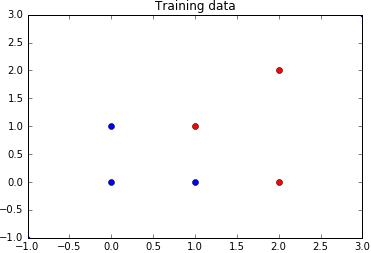
\includegraphics[page=1,width=0.60\textwidth]{diagram.png}
	\caption{\label{fig:diagram}{Hehehe}}
\end{figure}

\begin{lstlisting}[frame=single]
for i:=maxint to 0 do
begin
{ do nothing }
end;
Write('Case insensitive ');
Write('Pascal keywords.');
\end{lstlisting}

\end{document}